\documentclass[tikz,border=10pt]{standalone}
\usepackage{tikz}

\begin{document}
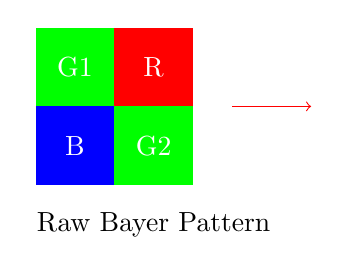
\begin{tikzpicture}

% Define the size of each square
\def\squaresize{1cm}
\def\patternsize{4}

% Draw the Bayer pattern
\begin{scope}[shift={(0,0)}]
% Loop to draw the squares
\foreach \i in {0,1} {
    \foreach \j in {0,1} {
        \pgfmathtruncatemacro{\row}{mod(\i, 2)}
        \pgfmathtruncatemacro{\col}{mod(\j, 2)}
        
        % Choose color based on position
        \ifnum \row=0
            \ifnum \col=0
                \def\fillcolor{blue}
                \def\textcolor{white}
                \def\label{B}
            \else
                \def\fillcolor{green}
                \def\textcolor{white}
                \def\label{G1}
            \fi
        \else
            \ifnum \col=0
                \def\fillcolor{green}
                \def\textcolor{white}
                \def\label{G2}
            \else
                \def\fillcolor{red}
                \def\textcolor{white}
                \def\label{R}
            \fi
        \fi

        % Draw the square
        \fill[\fillcolor] (\i,\j) rectangle ++(1,1);
      \node[text=\textcolor] at (\i*\squaresize+0.5*\squaresize, \j*\squaresize+0.5*\squaresize) {\label}; 
    }
    }
  % Label the Bayer pattern
  \node at (1.5*\squaresize,-0.5) {Raw Bayer Pattern};
\end{scope}
\draw[->,red] (2.5,1) -- (3.5,1);
% Draw the demosaicing process - highlighting a 2x2 square

\end{tikzpicture}
\end{document}
